\documentclass[10pt]{article}
\usepackage[utf8]{inputenc}
\usepackage{url}
\usepackage{hyperref}
\usepackage{amsmath}
\usepackage{amsfonts}
\usepackage{amssymb}
\usepackage{graphicx}
\graphicspath{ {./images/} }
\usepackage{float}
\usepackage{lipsum}
\usepackage{sectsty}
\sectionfont{\centering}
\usepackage{multicol}
\usepackage{xcolor}
\usepackage{natbib}
\usepackage{graphicx}
\usepackage{listings}
\usepackage{xcolor}
\usepackage[font=small]{caption}
\addtolength{\abovecaptionskip}{-3mm}
\addtolength{\textfloatsep}{-5mm}
\setlength\columnsep{20pt}

\usepackage[a4paper,left=1.50cm, right=1.50cm, top=2cm, bottom=3cm]{geometry}


\author{}

\title{\Large{Design and Analysis of Algorithms Assignment - 5}}

\begin{document}
	
	\begin{center}
		{\Large \textbf{Design and Analysis of Algorithms Assignment - 5}}\\
		\vspace{1em}
		{\large Department of Information Technology,}\\
		\vspace{1em}
		\large{Indian Institute of Information Technology, Allahabad 211015, India}\\
		\vspace{1em}
		\large{Sainath Reddy (IIT2019201), Jyoti Verma(IIT2019202), Krishna Kaipa(IIT2019203)}
		\vspace{2.5em}
		
	\end{center}
	
\begin{multicols*}{2}

    \textbf{\emph{{Abstract}: The longest Zig-Zag subsequence problem is to find length of the longest subsequence of given sequence such that all elements of this are alternating.}}\\
	
	\textbf{\emph{{Index Terms}: Arrays, Dynamic Programming, Longest Subsequence}}

\section*{INTRODUCTION}
 
In this problem, we have to find the length of the longest subsequence of a given sequence such that the elements of this sequence are in alternating order.

\paragraph{Dynamic Programming}
The idea here is to apply dynamic programming. Dynamic programming: it was an optimization over a plain recursive algorithm. The idea here is to simply store the results of subproblems, so that we do not have to re-compute them when needed later.this simple optimization reduces time complexities from exponential to polynomial.


\paragraph{Algorithmic Steps:}

Our approach to implementing the solution and solving the problem is as follows:
\begin{enumerate}

\item We are going to take a dp as 2D array with  size  as 2*size of the given elements.The 2D array was going to have only two rows one is to store the length of longest alternating order and the other is to store the sign whether the present element in the sequence is greater than the previous or lesser than the previous element in the sequence. 

\item The sign has three values if the sign was -1 it means it was not taken part of any sequence (itself it was a sequence of length 1) and if the sign was 0 it means that the element was taken in some sequence and this element is lesser than the preceding element in the sequence. And 1 means that the element is taken in some sequence and this element was greater than the preceding element in the sequence.

\item In this way, we store the longest alternating sequence which ends at present element in the 1st row of 2D array and the sign in 2nd row of 2D array and we take the max of 1st row of 2D array which is same as  max length of alternating sequence.

\end{enumerate}

The above returned count is the longest alternating subsequence.

\paragraph{Code:}
\paragraph{Code:}
\lstset { %
    language=C++,
    backgroundcolor=\color{black!5},
    basicstyle=\footnotesize,
}


\begin{lstlisting}
#include <bits/stdc++.h>
using namespace std;

int main()
{
 int arr[100];
 cout<<"Enter number of elements to generate: ";
 int n;
 cin>>n;
 out<<endl;
 cout<<"Randomly generated array: "; 
 for(int i=0;i<n;i++)
 {
  arr[i] = rand() % 50 + 1;
  cout<<arr[i]<<" ";
}
	

int dp[n][2];

for(int i=0;i<n;i++)
{
 //minimum length 1
 dp[i][0] = 1; 
 //not part of a subsequence yet
 dp[i][1] =-1; 
}
int ma = 1;
for(int i=1;i<n;i++)
{
 int len =1;
 int dec=-1;
 for(int j=0;j<i;j++)
 {
   if(arr[j] < arr[i])
   {
     dec = 1;
     if(dp[j][0] >= dp[i][0])
     {
      if(dp[j][1] == -1 || dp[j][1] == 0) 
      //was lesser than its previous element
      {
        len = max(len,dp[j][0]+1);
      }
     }
    }
    else if(arr[j] > arr[i])
    {
      dec = 0;
      if(dp[j][0] >= dp[i][0])
      {
        if(dp[j][1] == -1 || dp[j][1] == 1) 
        //was greater than its previous element
        {
          len = max(len,dp[j][0]+1);
        }
      }
    }
 }
 dp[i][1] = dec;
 dp[i][0]  = len;
 ma = max(ma,dp[i][0]);
}
    
cout<<"\nLength of longest subsquence is: "<<ma;
return 0;
}
\end{lstlisting}
\section*{ANALYSIS}

\paragraph{Apriori Analysis:}   
This is the analysis performed prior to running in a stage where the function is defined using a theoretical model. Therefore, complexity is determined by just examining the algorithm rather than running it on a particular system with a different memory,processor, and compiler. 
\begin{enumerate}

\item Time Complexity.

The time complexity of the DP approach is $ O(n^2). $ \\
For each element at index i we have to check it with each and every element which are preceding it. As there is a possibility that it can be added with any of preceding elements in order to get the longest altering sequence.

So for each i we have to do (i-1) checks and there are n elements so the time complexity was going to be  $ O(n^2). $\\

\item Space Complexity.

The space complexity of the DP approach is o(n) as we are talking a 2D array with size 2*no elements of sequence as the size.
Space complexity : O(n)

\end{enumerate}

\paragraph{Aposteriori Analysis:}

Aposteriori analysis of an algorithm means we per- form analysis of an algorithm only after running it on a system. It directly depends on the system and changes from system to system.So for the a aposteriori analysis of the algorithm,we have run our code on the compiler and get values of the time.

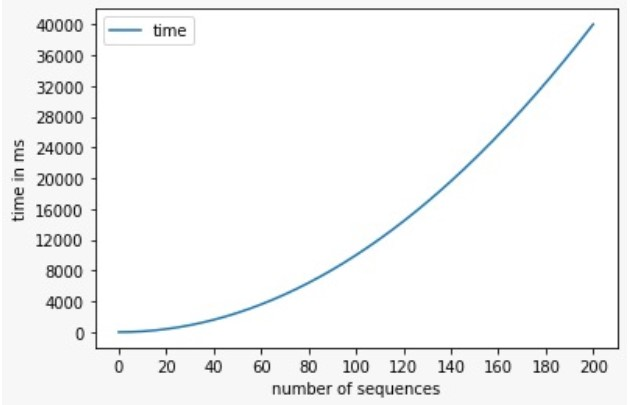
\includegraphics[width=\columnwidth, height=8cm]{time.jpg}\begin{center}\textbf{Figure 1:} Time Complexity\end{center}

\section*{APPLICATIONS}
Some of the applications of the Dynamic Progamming Approach are:

\begin{enumerate}
\item 0/1 knapsack problem
\item Mathematical optimization problem
\item All pair Shortest path problem
\item Reliability design problem
\item Longest common subsequence (LCS)
\item Flight control and robotics control
\end{enumerate}

\section*{CONCLUSION}

In this paper, we had discussed an algorithm which can be used to find the largest alternating subsequence in the given sequence. In this method we had used a dynamic programming approach by storing the answers of the subproblems and using them to solve the answer. The time complexity of this algorithm is $ O(n^2) $ and space complexity is O(n).

\section*{REFERENCES}

\begin{enumerate}
\item Introduction to Dynamic Programming Technique:\\
https://www.geeksforgeeks.org/dynamic-programming/
\item Introduction to Algorithms by Cormen,Charles, Rivest and Stein.\\
https://web.ist.utl.pt/~fabio.ferreira/material/asa
\end{enumerate}



\newpage
\section*{APPENDIX}
\textbf{To run the code, follow the following procedure:}\\
\begin{enumerate}
    \item Save the code with your own desirable name and extension is .cpp
    \item Open the code with any IDE like Sublime Text, VS Code, Atom or some online compilers like GDB.
    \item Run the code following the proper running commands(vary from IDE to IDE)
    \begin{enumerate}
        \item \textbf{For VS Code:} Press Function+F6 key and provide the input on the terminal.
        \item \textbf{For Sublime Text:} Click on the Run button and provide the input.\\
    \end{enumerate}
\end{enumerate}
\end{multicols*}
	
\end{document}